\documentclass[tikz]{standalone}

% Font
\usepackage{mathpazo}
\usepackage{libertine}
\renewcommand*\sfdefault{phv}

\large

% Color
\usepackage{xcolor}
\definecolor{f1}{HTML}{F39019}
\definecolor{b1}{HTML}{DE6A10}
\definecolor{f2}{HTML}{51A7F9}
\definecolor{b2}{HTML}{0365C0}
\definecolor{f3}{HTML}{70BF41}
\definecolor{b3}{HTML}{00882B}

% tikz
\usepackage{tikz}
\tikzstyle{every node}=[font=\sffamily]
\usetikzlibrary{shapes,arrows,positioning,calc,decorations.markings,backgrounds}
\tikzstyle{c1} = [thick,draw=b1,fill=f1]
\tikzstyle{c2} = [thick,draw=b2,fill=f2]
\tikzstyle{c3} = [thick,draw=b3,fill=f3]
\tikzstyle{cg} = [thick,draw=gray!50,fill=gray!30]
\tikzstyle{rect} = [rectangle, minimum height=1cm]
\tikzstyle{roundrect} = [rect, rounded corners=.2cm]
\tikzstyle{io} = [trapezium, trapezium left angle=70, trapezium right angle=110]
\tikzstyle{arrow} = [thick,->,>=stealth]

\tikzstyle{sm} = [roundrect, c1, minimum height=0.8cm]
\tikzstyle{data} = [io, cg, text width=1.8cm, align=center]

\begin{document}
	
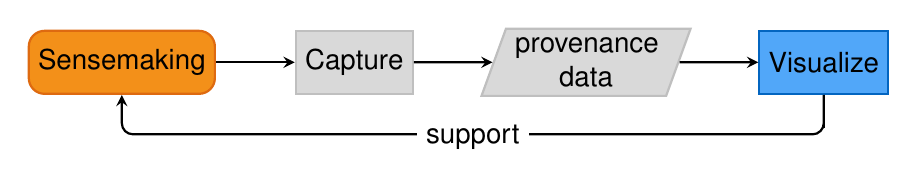
\begin{tikzpicture}[node distance=1cm, auto]
\node (sm) [sm] {Sensemaking};
\node (capture) [cg, rect, minimum height=0.8cm, right=of sm] {Capture};
\node (data) [data, right=of capture] {provenance data};
\node (vis) [c2, rect, minimum height=0.8cm, right=of data] {Visualize};
%\node (reuse) [ap, right=of vis] {Reuse};

\draw [arrow] (sm) -- (capture);
\draw [arrow] (capture) -- (data);
\draw [arrow] (data) -- (vis);
%\draw [arrow] (vis) -- (reuse);
\draw [arrow, rounded corners] (vis.south) |- ++(0,-0.5) -| (sm.south); 
\node [rectangle,fill=white,inner ysep=0,yshift=-.95cm] at ($(vis)!0.5!(sm)$) {support};
\end{tikzpicture}
	
\end{document}